%%  Codeing: utf8

\documentclass{mcmthesis}

\mcmsetup{CTeX=true,
			tcn = 12138, problem = C,
			sheet = true, titleinsheet = true, keywordsinsheet = true,
			titlepage = true, abstract = false}

\usepackage{palatino}

\usepackage{lipsum}			%随机生成一段文本
\usepackage{amsmath}
%\usepackage{amslatex}		%没有
\usepackage[UTF8, nocap]{ctex}

\usepackage{hyperref}

\title{Our title}
\author{ly}
\date{\today}
%\date{Jan. 20$^{\text{th}}$}

%\author{\small \href{http://www.latexstudio.net/}
% {
\includegraphics[width=7cm]{mcmthesis-logo}}}
%\date{\today}

 %正文摘要和控制页摘要名字修改
%\def\abstractname{Abstract}
%\def\sheetsummaryname{Summary}

\begin{document}

\begin{sheetsummary}
\lipsum[1]
asdasdasd\\
\date{\today}
\end{sheetsummary}

\begin{keywords}
keyword1, keyword2
\end{keywords}

\maketitle
\tableofcontents
\newpage

\section{Introduction}
\lipsum[3]
Ru guo ni bu xiang xian shi zhe duan wen zi, qing ba \textit{lipsum} shanchu.\\
如果你不想显示上面的那段文字,那就把 \textit{lipsum}删掉
获得更多的latex教材,请添加latex交流群,或者关注迈思数模微信公众号:shumohome并回复“LATEX资料”
美赛LATEX模板交流群:193607493
啊睡觉的卡拉胶斯科拉金龙客车那看来寄售点卡了就是打老师的空间看了就疯狂拉升那份感觉快乐撒ui顿撒酒疯能接受
This is the best model of the Problem.\\

\begin{itemize}
\item Minimizes the discomfort to the hands, or
\item Maxmize the outgoing velocity of the ball.
\item
\end{itemize}
We focus it .
\begin{Theorem} \label{thm:tex}
\LaTeX
\end{Theorem}
\begin{Lemma} \label{thm:tex}
\TeX
\end{Lemma}
\begin{proof}
The proof of theorem.
\end{proof}

\date{\today}
\date{Jan. 20$^{\text{th}}$}
\subsection{Other Assumption}
其他假设\\


\begin{itemize}
\item 
\item
\item
\end{itemize}


\section{Analysis of the Problem}
analysis\\
\begin{figure}[h]
%\small
\centering
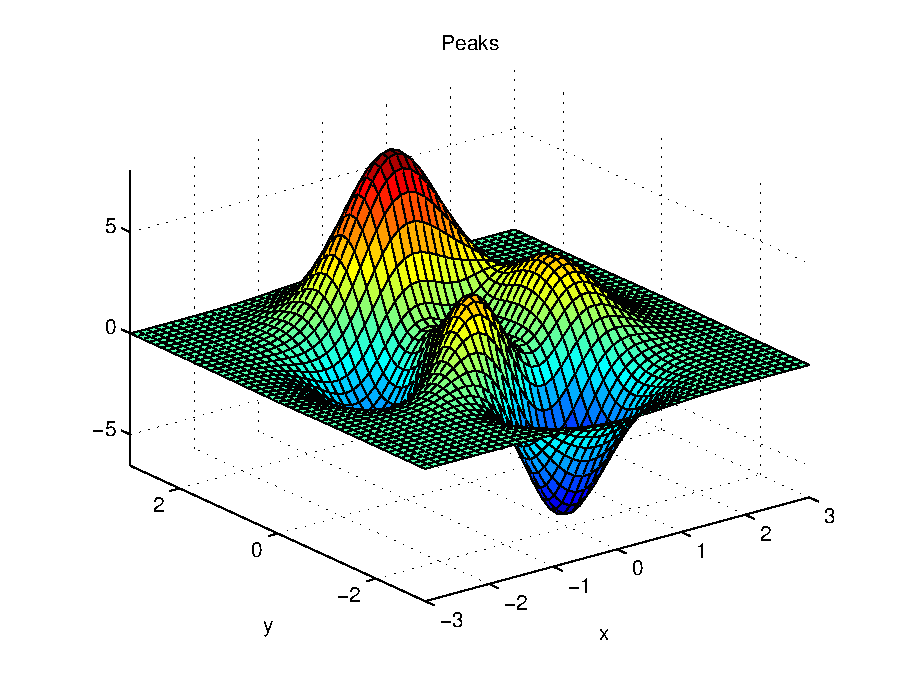
\includegraphics[width = 12cm]{mcmthesis-aaa.eps}
\caption{Figure example 1}	\label{fig:aa}
\end{figure}

\lipsum[5] \eqref{aa}\\				%???????????????????????????
Figure \ref{aa}.

\begin{figure}[h]
\begin{minipage}[h]{0.5\linewidth}
\centering

\includegraphics[width = 0.8\textwidth]{0.jpg}
\caption{Figure example 2}
\end{minipage}
\begin{minipage}[h]{0.5\linewidth}
\centering

\includegraphics[width = 0.8\textwidth]{0.jpg}
\caption{Figure example 3}
\end{minipage}
\end{figure}

\lipsum[5]

\begin{equation}
E = m \cdot c^2
\end{equation}

\[\left( {\begin{array}{*{20}{c}}
  {*20c{a_{11}}}&{{a_{12}}}&{{a_{13}}} \\ 
  {{a_{21}}}&{{a_{22}}}&{{a_{23}}} \\ 
  {{a_{31}}}&{{a_{32}}}&{{a_{33}}} 
\end{array}} \right) = \frac{{Opposite}}{{Hypotenuse}}{\cos ^{ - 1}}\theta \arcsin \theta \]
\lipsum[6]
\[
{p_j} = \begin{cases} 0, &\text{if $j$ is odd}\\
r!\,(-1)^{j/2}, &\text{if $j$ is even}
\end{cases}
\]

\lipsum[7]
\[
\arcsin \theta  = \mathop{{\int\!\!\!\!\!\int\!\!\!\!\!\int}\mkern-31.2mu \bigodot}\limits_\varphi  
 {\mathop {\lim }\limits_{x \to \infty } \frac{{n!}}{{r!(n - r)!}}} 	\eqno (1)			%设置公式的编号
\]


\section{Calculating and Simplifying the Model  }
Model\------模型\\
\lipsum[8]
$\mathop{A}_{ij}$ and ${A}_{ij}$ 不一样

$\left(123 \right)$ and $ (123) $ and (123) 不一样


\section{The Model Results}
\lipsum[4]

\section{Validating Model}

\begin{center}
\begin{tabular}{c|cclcrcc}
\hline
\hline
Year & theta & $S_1^-$ & $S_2^-$ & $S_3^-$ & $S_4^+$ & $S_5^+$ & $S_6^+$ \\			%表头
\hline
2016 & 1      & 0      & 0 & 0.0001 & 0      & 0      & 0 \\
2017 & 0.9997 & 0.0555 & 0 & 0.2889 & 0.1844 & 0.463  & 0 \\
2018 & 0.9994 & 0      & 0 & 0.0012 & 0.3269 & 0.7154 & 0 \\
2019 & 0.9993 & 0      & 0 & 0      & 0.4325 & 1.0473 & 0 \\
2020 & 0.9991 & 0      & 0 & 0      & 0.5046 & 1.2022 & 0 \\
2021 & 0.999  & 0      & 0 & 0      & 0.5466 & 1.2827 & 0 \\
2022 & 0.9989 & 0.0017 & 0 & 0.3159 & 0.562  & 1.2995 & 0 \\
2023 & 0.9989 & 0      & 0 & 0.0109 & 0.5533 & 1.2616 & 0 \\
2024 & 0.9989 & 0      & 0 & 0      & 0.5232 & 1.1769 & 0 \\
2025 & 0.9989 & 0      & 0 & 0.1009 & 0.4738 & 1.0521 & 0 \\
2026 & 0.9991 & 0      & 0 & 0      & 0.4071 & 0.8929 & 0 \\
2027 & 0.9992 & 0.0004 & 0 & 0.1195 & 0.3248 & 0.7042 & 0 \\
2028 & 0.9994 & 0.0164 & 0 & 0.046  & 0.2287 & 0.4902 & 0 \\
2029 & 0.9997 & 0      & 0 & 0.0609 & 0.12   & 0.2545 & 0 \\
2030 & 1      & 0      & 0 & 0      & 0      & 0      & 0 \\
\hline
\hline
\end{tabular}
\end{center}

\section{Conclusions}
\lipsum[5]

\begin{center}
\begin{tabular}{c|cc}
\hline
年份 & \multicolumn{2}{c}{指标} \\
\hline
2017 & 0.9997 & 0.0555 \\
2018 & 0.9994 & 0      \\
2019 & 0.9993 & 0      \\
\hline
\end{tabular}
\end{center}

\lipsum[3]
\begin{table}[h]
\centering
\begin{tabular}{c|cc}
\hline
年份 & \multicolumn{2}{c}{指标} \\
\hline
2017 & 0.9997 & 0.0555 \\
2018 & 0.9994 & 0      \\
2019 & 0.9993 & 0      \\
\hline

\end{tabular}
\caption{NAME}\label{SIGN}
\end{table}

Let's to see Table \ref{SIGN}.

\begin{minipage}{0.5\linewidth}
\begin{tabular}{|c|c|c|}
\hline
\multicolumn{2}{|c|}{\multirow{2}{*}{合并}} & 测试 \\
\cline{3-3}
\multicolumn{2}{|c|}{} & 0.9998 \\
\hline
2018 & 0.9998 & 0 \\
\hline
\end{tabular}
\end{minipage}
\begin{minipage}{0.5\linewidth}
\begin{tabular}{c|ccc}
\hline
年份 & \multicolumn{3}{c}{指标} \\
\hline
\multirow{3}{*}{合并} & 2017 & 0.9997 & 0.0555 \\
&2018 & 0.9994 & 0      \\
&2019 & 0.9993 & 0      \\
\hline
\end{tabular}
\end{minipage}








\section{A Summary}
\lipsum[7]

\-{A}    \^{b}\\
%\begin{displatmath}
%\bar{A}
%\end{displaymath}
\begin{math}
\bar{A} \quad \forall x \in \mathbf{R}
\end{math}
The asjdjj $\widehat{A}\qquad \exists Z \subset \mathbb{C}$

\section{Evaluate of the Model}
\lipsum[2]

\begin{equation}	\label{eq:eps}		%???不起作用
lim_{n \to \infty} f_{n}(x) = \frac{a}{b}
\end{equation}
\[\mathop {\lim }\limits_{n \to \infty } {f_n}(x) = \frac{a}{b}\]
\begin{equation}
\mathop {\lim }\limits_{n \to \infty } {f_n}(x) = \frac{a}{b}
\end{equation}

\eqref{eps}				%?????????????????????????


\section{Strengths and Weaknesses}
\subsection{Strengths}
\begin{itemize}
\item \textbf{Applies widely}\\
This  system can be used for many types of airplanes, and it also
solves the interference during  the procedure of the boarding
airplane,as described above we can get to the  optimization
boarding time.We also know that all the service is automate.
\item \textbf{Improve the quality of the airport service}\\
Balancing the cost of the cost and the benefit, it will bring in
more convenient  for airport and passengers.It also saves many
human resources for the airline. \item \textbf{}
\end{itemize}

\subsection{Weaknesses}
\begin{itemize}
\item
\item
\end{itemize}


\begin{thebibliography}{99}
\bibitem{1} \href{https://wenku.baidu.com/view/025f88e1b8f67c1cfad6b8bb.html}{D.~E. KNUTH   The \TeX{}book  the American
Mathematical Society and Addison-Wesley
Publishing Company , 1984-1986.}
\bibitem{2}\href{https://openknowledge.worldbank.org/handle/10986/2959}{Lamport, Leslie,  \LaTeX{}: `` A Document Preparation System '',
Addison-Wesley Publishing Company, 1986.}
\bibitem{3}\url{http://www.chinatex.org/}
\bibitem{4} UK. Department for Transport. The Highway Code. N.p., 5 Dec. 2016. Web. 21 Jan. 2017. Available:\quad\href{ https://www.gov.uk/guidance/the-highway-code/general-rules-techniques-and-advice-for-all-drivers-and-riders-103-to-158#rule126}{https://www.gov.uk/guidance/the-highway-code/general-rules-techniques-and-advice-for-all-drivers-and-riders-103-to-158\#rule126.}
\bibitem{5}\url{http://www.4399.com/}
\end{thebibliography}


\begin{appendices}

\section{First appendix}
\lipsum[4]

Here are simulation programmes we used in our model as follow.\\

\textbf{\textcolor[rgb]{0.98, 0.00, 0.00}{Input matlab source:}}
\lstinputlisting[language = matlab]{./code/mcmthesis-matlab1.m}

\section{Second appendix}
\quad\quad \textcolor[rgb]{0.98, 0.00, 0.00}{\textbf{Input C++ source:}}
\lstinputlisting[language = C++]{./code/mcmthesis-sudoku.CPP}

\section{Third appendix}
Some more text \textcolor[rgb]{0.98, 0.00, 0.00}{\textbf{Input Python sources:}}
\lstinputlisting[language = Python]{./code/Quicksort.py}

\end{appendices}

%\end{document}
\end{document}


%%
%% This work consists of these files mcmthesis.dtx,
%%                                   figures/ and
%%                                   code/,
%% and the derived files             mcmthesis.cls,
%%                                   mcmthesis-demo.tex,
%%                                   README,
%%                                   LICENSE,
%%                                   mcmthesis.pdf and
%%                                   mcmthesis-demo.pdf.
%%
%% End of file `mcmthesis-demo.tex'.
